% The master file of dissertation
\documentclass[]{gwthesis}

\usepackage{amssymb}
\usepackage{amsmath}
\usepackage{cases}
\usepackage{tabularx}
\usepackage{color}
\usepackage{enumerate}
%\usepackage{slashbox}
\usepackage{caption}
\usepackage{mathtools}



\begin{document}

% Title page
\title{A New Finite Element Method Enabling Parallel Solutions for Second Order Elliptic Equation}
\author{Bin Zhang}
\prevdegrees{B.S. in Mechanics, June 2009, University of Science and Technology of China \\
             M.S. in Aerospace Engineering, August 2012, University of Notre Dame}
\school{The School of Engineering and Applied Science}
\institution{The George Washington University}
\degree{Doctor of Philosophy}
\degreeyear{2016}
\degreemonth{August}
\degreeday{31}
\defensedate{July 22, 2016}
\advisorname{Chunlei Liang}
\advisortitle{Associate Professor of Engineering and Applied Science}
\committeea{Chunlei Liang, Associate Professor of Engineering and Applied Science, Dissertation Director}
\committeeb{Michael Plesniak, Professor of Engineering and Applied Science, Committee Member}
\committeec{Charles Garris, Professor of Engineering and Applied Science, Committee Member}
\committeed{Murli Gupta, Professor of Mathematics, Committee Member}
\committeee{Johan Larsson, Assistant Professor of Mechanical Engineering, University of Maryland, College Park, Committee Member}
\committeef{David Kopriva, Professor of Mathematics, Florida State University, Committee Member}

\maketitle

% frontmatter
\begin{frontmatter}
  \approvalpage
  \copyrightpage
  \begin{dedication}

I dedicate this work to my family, for their boundless love.

\end{dedication}

  \begin{acknowledgements}

I am deeply thankful for my advisor, Professor Chunlei Liang. His broad knowledge inspired me, his restless hardworking  encouraged me, his constant advice enlightened me and his generous support helped me through my whole graduate study at the George Washington University. It is my best grateful to have Dr. Junping Wang, a pioneer of weak Galerkin finite element method, as my co-advisor. His works inspire numerous researchers and point a promising direction for the following study. I would like to thank to all committee members, Dr Lin Mu, Prof. Adam Wickenheiser, Prof. Murli Gupta for their insightful advice on this piece of work. Additional thanks for the research group partners and best friends: Junfeng, Bin, Jingjing, Xiaoliang, Mao, Zihua, Zhen and Rongguang.

\end{acknowledgements}s

  \begin{abstract}
In this paper, we present a novel parallel computing method to efficiently solve linear elasticity problems on unstructured meshes. The implementation of our parallel method is based on the weak Galerkin (WG) finite element method which has been recently developed by Wang and Ye, et al. The weak Galerkin finite element method refers to a general finite element method to solve partial differential equations. The core idea of utilizing WG method on solving linear elasticity equation is converting the weak strain and stress tensors  the concept of discrete weak gradients. The main feature is that the differential operators are calculated through the newly developed weak functions and then reconstructed by solving the elemental matrices on each element with lower computational cost.

Linear elasticity is the equation describes how solid objects stress and strain distribute due to the external and internal prescribed loading conditions. This equation requires the materials as continua. On the purpose of solving large-scale fluid structure interaction problems, we are in favor of the partitioned approach as the high order accuracy perspective. In this scheme, the governing equation for fluid and displacement of the structure are calculated in two different solver. An in-house high order accuracy fluid solver for Naiver-Stokes equations is ready to use. We now present an accurate and efficient solid solver which is compatible with that on solving large scale fluid structural interaction problems..

To enable parallel computation, the entire computational domain is divided into arbitrary number of subdomains.We present two different approaches to implement the parallel computing. Firstly, we combine the classic continuous Galerkin (CG) finite element with weak Galerkin (WG) finite element method together and develop a hybrid element. The hybrid element inherit the discontinuous feature from WG method and the computational efficiency from CG method. 
The other method is to implement the duality concept to split the computational space into primal and dual spaces. The connection of adjacent subdomains is implemented through the balancing domain decomposition with constraints (BDDC) which was originally proposed in\cite{mandel1993balancing}. Locally over each subdomain, matrices are constructed for interior and interface quantities separately. Subsequently, interface related matrices are passed over to their adjacent subdomains through inter-processor communication library (MPI). 

In Chapter 1, we introduce the background and meaning for this thesis. We provide the preliminaries which are necessary for the following presentation. We derived the bilinear form of second order elliptical equation and linear elasticity equation. 

In Chapter 2, we discuss the weak Galerkin finite element method and the bilinear form of linear elasticity equation.The WG finite element method is based on the variational form of equations. It is compatible for general polygons on a finite element computational domain. The computational matrix derived from WG method is symmetric and positive definite. Due to the flexibility of the polynomials basis functions, it's convenient to obtain high order accuracy solutions. The convergence rate for WG method is bounded by the lowest order.

In Chapter 3, we design a novel parallel computing method to efficiently solve elastic equation. The core idea of the WG method for solving linear elastic equation is to replace its gradients after the integration by parts by discrete weak strain and stress tensors. We develop a novel hybrid element which combines the elements of both weak Galerkin (WG) finite element method and continuous Galerkin (CG) finite element method. The new hybrid element inherits the discontinuous feature of the WG method. We insert an arbitrary number of CG elements in one single WG element. The hybrid element provides a second order of accuracy for both linear and nonlinear elastic equation. The superlinear speedup is observed.

In Chapter 4, we develop a novel parallel computing method to efficiently solve linear elasticity problems on unstructured meshes. The core idea of the WG method for solving linear elasticity equation is to introduce weak strain and stress tensors by using the concept of discrete weak gradients. To enable parallel computation, the computational grid is split into arbitrary number of subdomains. The connection of adjacent subdomains is realized through the balancing domain decomposition with constraints (BDDC) which was originally proposed in \cite{mandel1993balancing}. Locally over each subdomain, matrices are constructed for interior and interface quantities separately. Subsequently, interface related matrices are passed over to their adjacent subdomains through MPI. MPI communications are used to help construct a smaller global matrix leaving most of computational operations locally to each processor. The designed WG-BDDC parallel algorithm achieves outstanding scalability by testing over 600 processors. Our numerical results also demonstrate that the WG-BDDC method pos- sesses designed orders of accuracy for both 2nd-order and 3rd-order spatial discretization schemes. Moreover, condition numbers for all test problems are well bounded demonstrating the stability of WG-BDDC method for parallel processing.

In Chapter 5, we present computational fluid dynamics (CFD) simulations of the blood flow in stenotic arteries with idealized geometries. These arteries are typically simplified as axisymmetric constriction in straight tubes. The hydrodynamics of blood flow in these arteries are modeled using unsteady incompressible Navier-Stokes equations. The 3D computational domain is represented by unstructured meshes with all hexahedral elements. An efficient pressure-based Finite Volume Method(FVM)\cite{liang2007large} was implemented to solve these equations. Our simulations include computational geometries with a wide range of narrowing degrees of stenoses, from 40\% to 80\% luminal area reduction. The number of stenoses ranges from 1 to 7. Several different spatial intervals were considered between adjacent stenoses. The upstream flow condition was implemented by using measured peripheral artery flow which at the Reynolds number of 500.

In Chapter 6, We conclude the current stage and explore the future potential work.

\textbf{Keyword} : weak Galerkin, finite element method, parallel computing, linear elasticity, message passing interface, continuous Galerkin, domain decomposition, balancing domain decomposition by constraints, polygonal meshes

\end{abstract}

  \tableofcontents \clearpage
  \listoffigures   \clearpage
  \listoftables
\end{frontmatter}


% chapters
\chapter{Introduction}
\label{ch:chap1}


%------------------------------------------
\section{Backgrounds}

\subsection{Engineering Background}

Peripheral artery disease (PAD) is a major cause of amputation in United States. It is prevalent among smokers, diabetics and patient with dyslipidemia. Meanwhile, the long waiting time and high expense are two major problems for the patients. In the modern clinic room, the doctors are eagerly looking for a solution which can provide high fidelity and high resolution images to help to analyze the PAD. The  present technology can only render and deliver two-dimensional,  monochrome, static and low-resolution picture. In recent decades, researchers contribute numerous effort on improving the diagnosis of stenoses and the quality of images\cite{clark1976fluid, nesbitt2009shear, wardlaw2006non, stergiopulos1992computer, long2001numerical}. With the fast development on both hardware and numerical method, the computational simulation can provide 3-D, dynamic, high resolution and fast scan results. Comparing to current CT scan, it's faster, cheaper and more accurate. Moreover, it's also very important that the simulation strategy can bring the doctors and patients that the dynamic growth animations of current stenoses and the following consequence after the clinic treatment. Fig \ref{fig: ch1f1} summarizes some factors which contributing to the interests in computational medical simulation technology\cite{barry2005features}. Many investigations have been conducted through last decades\cite{feng2012viscous, bertram2010evaluation, nadeem2010simulation, ogulu2005simulation}. However, since this is a fluid-structural interaction (FSI) problem, both high fidelity fluid and solid solver are needed. 

\begin{figure}[H]
	\centering
	\begin{tabular}{c}
		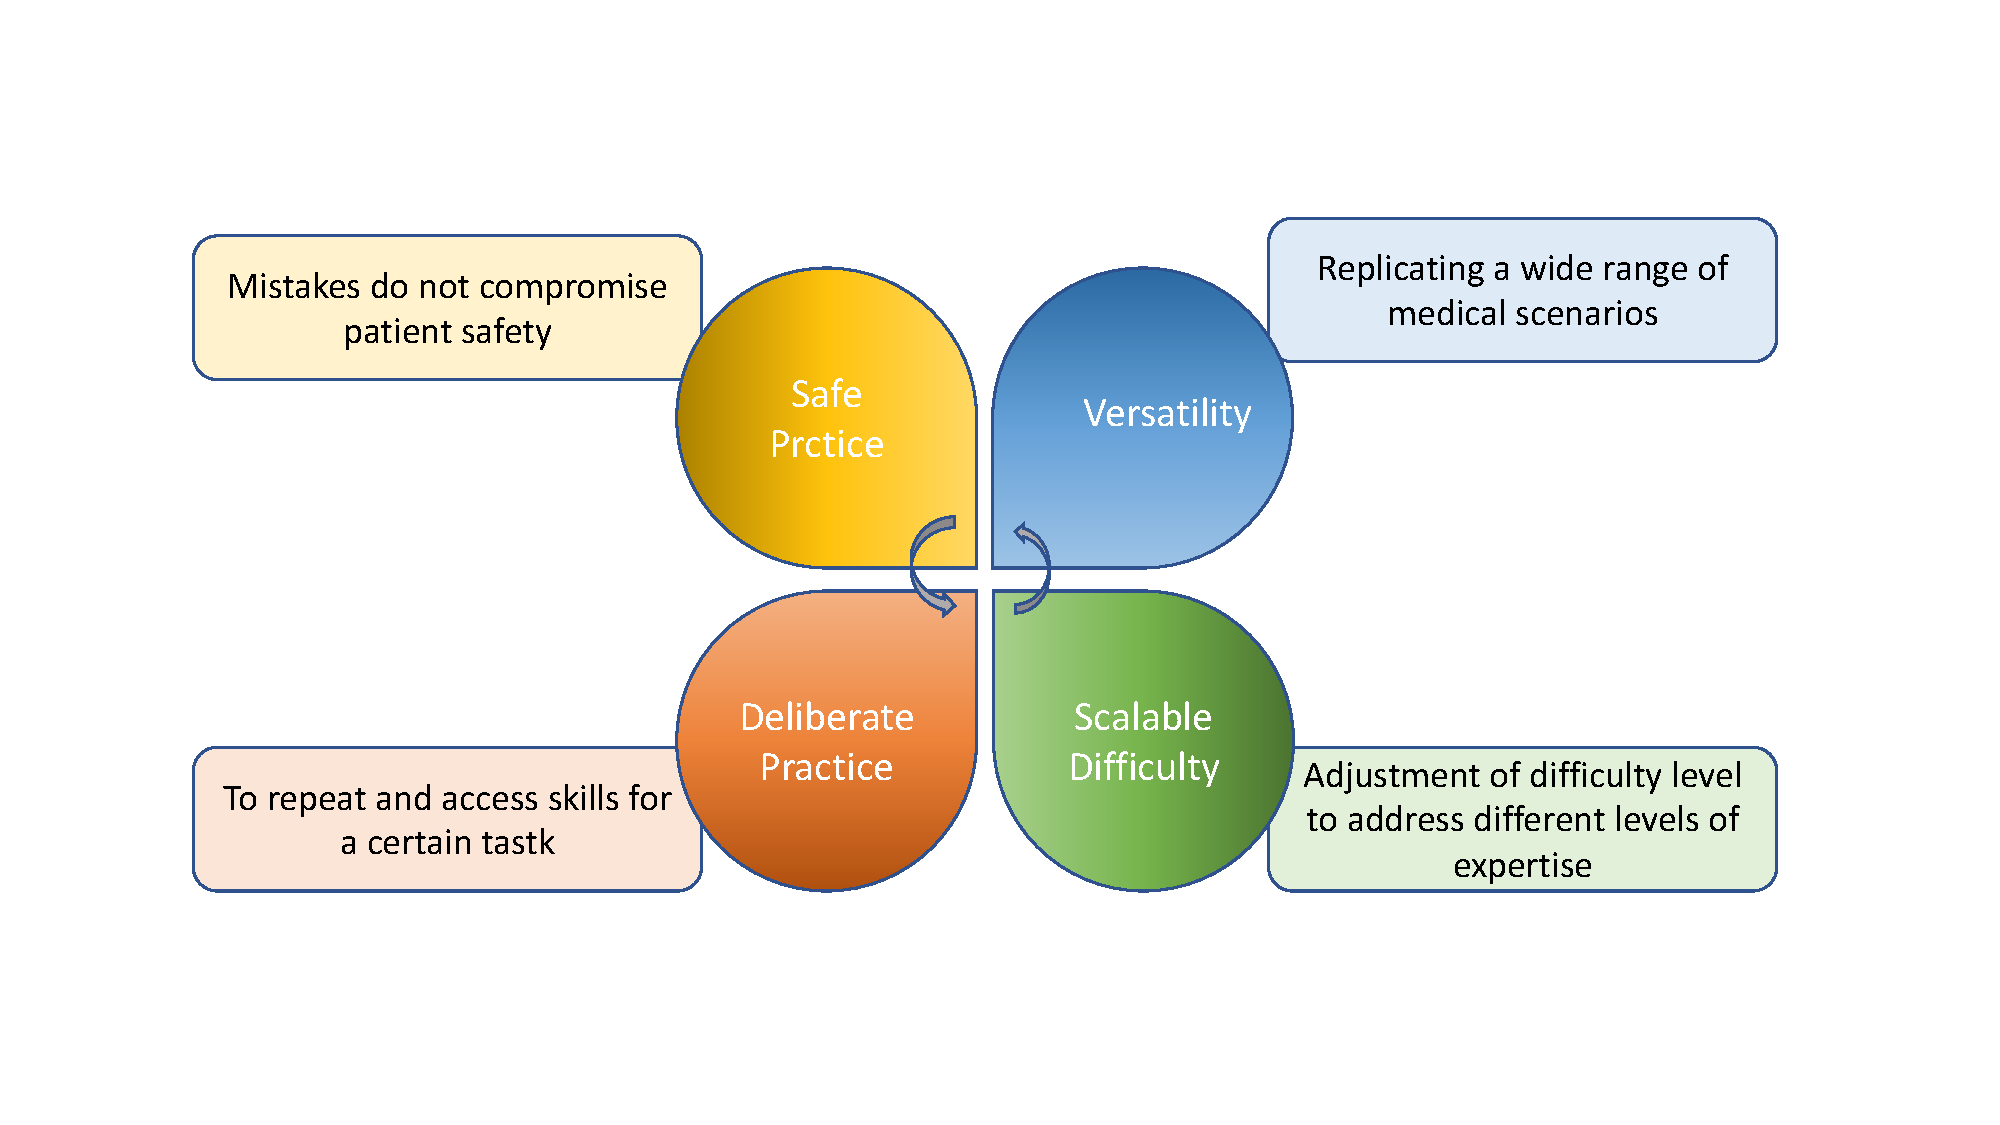
\includegraphics[width=1.0\textwidth]{./pics/computer_simulation}
	\end{tabular}
	\caption{\footnotesize Different factors affecting computer-based medical simulation.} \label{fig: ch1f1}
\end{figure}

The PAD can be abstracted as a fluid-structural interaction problem and be described by fluid and structure mathematic equations, respectively.  The two most popular approaches for solving FSI problems are monolithic method and partitioned method. For the monolithic approach, the two sets of equations, fluid and structural, are solved simultaneously. The mutual influence of each other can be considered directly. The obvious advantage of this scheme is simplicity. Only one global matrix is needed so that both the fluid and structural parts can be solved within the same space discretization and time marching scheme. On the contrary, we lose the flexibility to precisely control each partition. The other approach is partitioned method. The two sets of equations are solved separately and pass boundary conditions to each other like a cycle. The solution of fluid equations is calculated while the structural part is waiting for new input and vice versa. A coupling algorithm to exchange the interaction solution between two phases as a pair of modules. The Implicit-Explicit (IMEX) Runge-Kutta (RK) time integration approach has been proved the accuracy and efficiency on coupling the high order schemes\cite{zhang2016high}.

The high order parallel fluid solver \cite{liang2007large, liang2007large, liang2009effect} is accomplished and a series of CFD studies has been conducted along the ideal geometries. To implement the more realistic simulation, the tissue of blood vessel wall shall be considered as elastic material. Therefore, an accurate and efficient solver for elasticity equation is needed. The solver should be capable on calculating the material behavior according to the stiffness property, which is the response of the deformable model reacting to the external forces. The simplest model is mass-spring model which is easy to compute but can not accurately determine the material behavior. The other approach is finite element method, which is based on the continuum mechanics, has gained popularity since the results are more reliable. On the contrary to the mass-spring model, the FEM can specify the stiffness of the model by only using a few characteristic parameters, such as Young's modulus, Poisson ratio and the geometries. However, the challenges for FEM is very difficult to be used in real-time application due to the very high computational expense. 

\begin{figure}[H]
	\centering
	\begin{tabular}{c}
		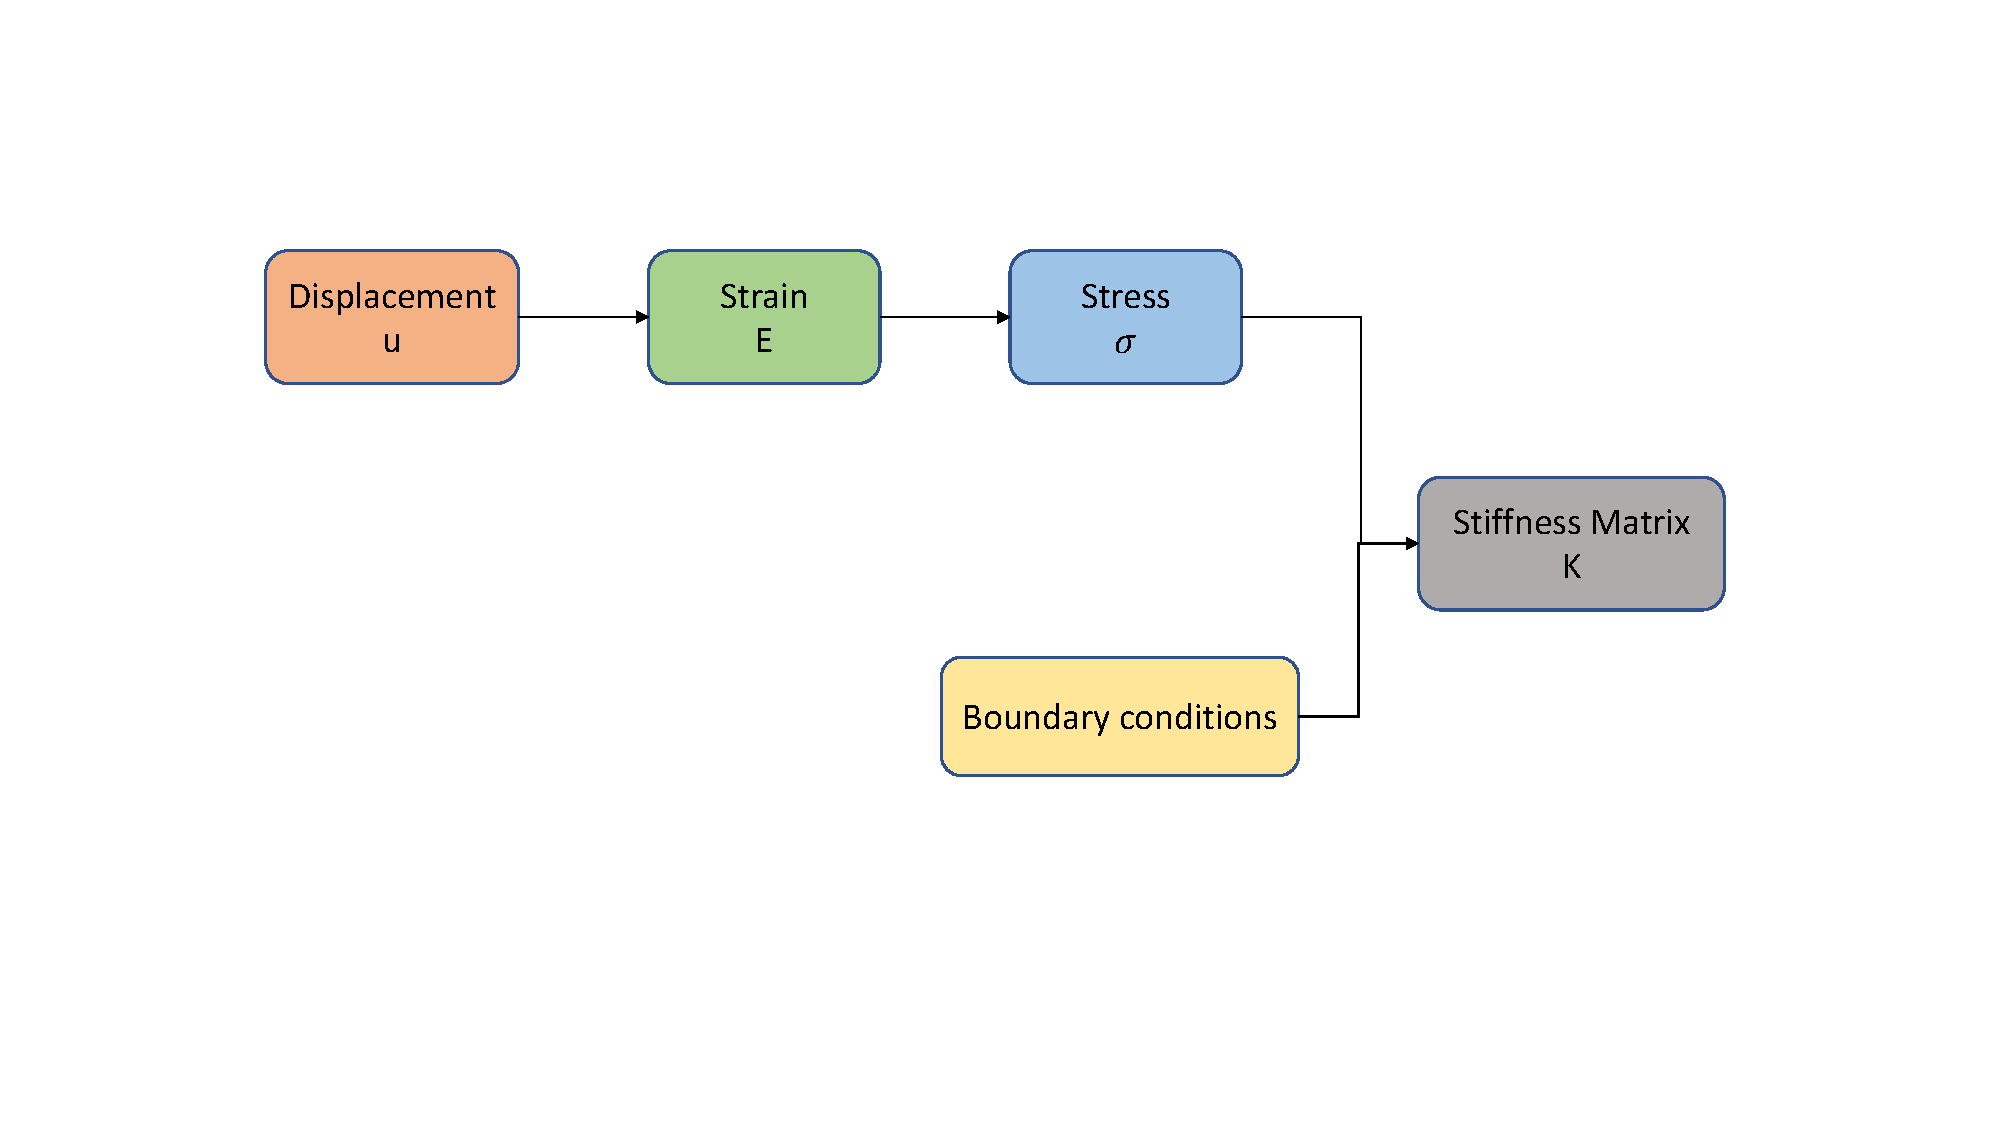
\includegraphics[width=1.0\textwidth]{./pics/construct_matrix}
	\end{tabular}
	\caption{\footnotesize Construct stiffness matrix.} \label{fig: ch1f2}
\end{figure}

Fig \ref{fig: ch1f2} shows a general process of calculating the stiffness matrix for a deformable material object. The stiffness matrix is derived from the gradient of stress which is calculated by the displacement and material property. The boundary conditions are imposed upon the contact interaction.

\begin{figure}[H]
	\centering
	\begin{tabular}{c}
		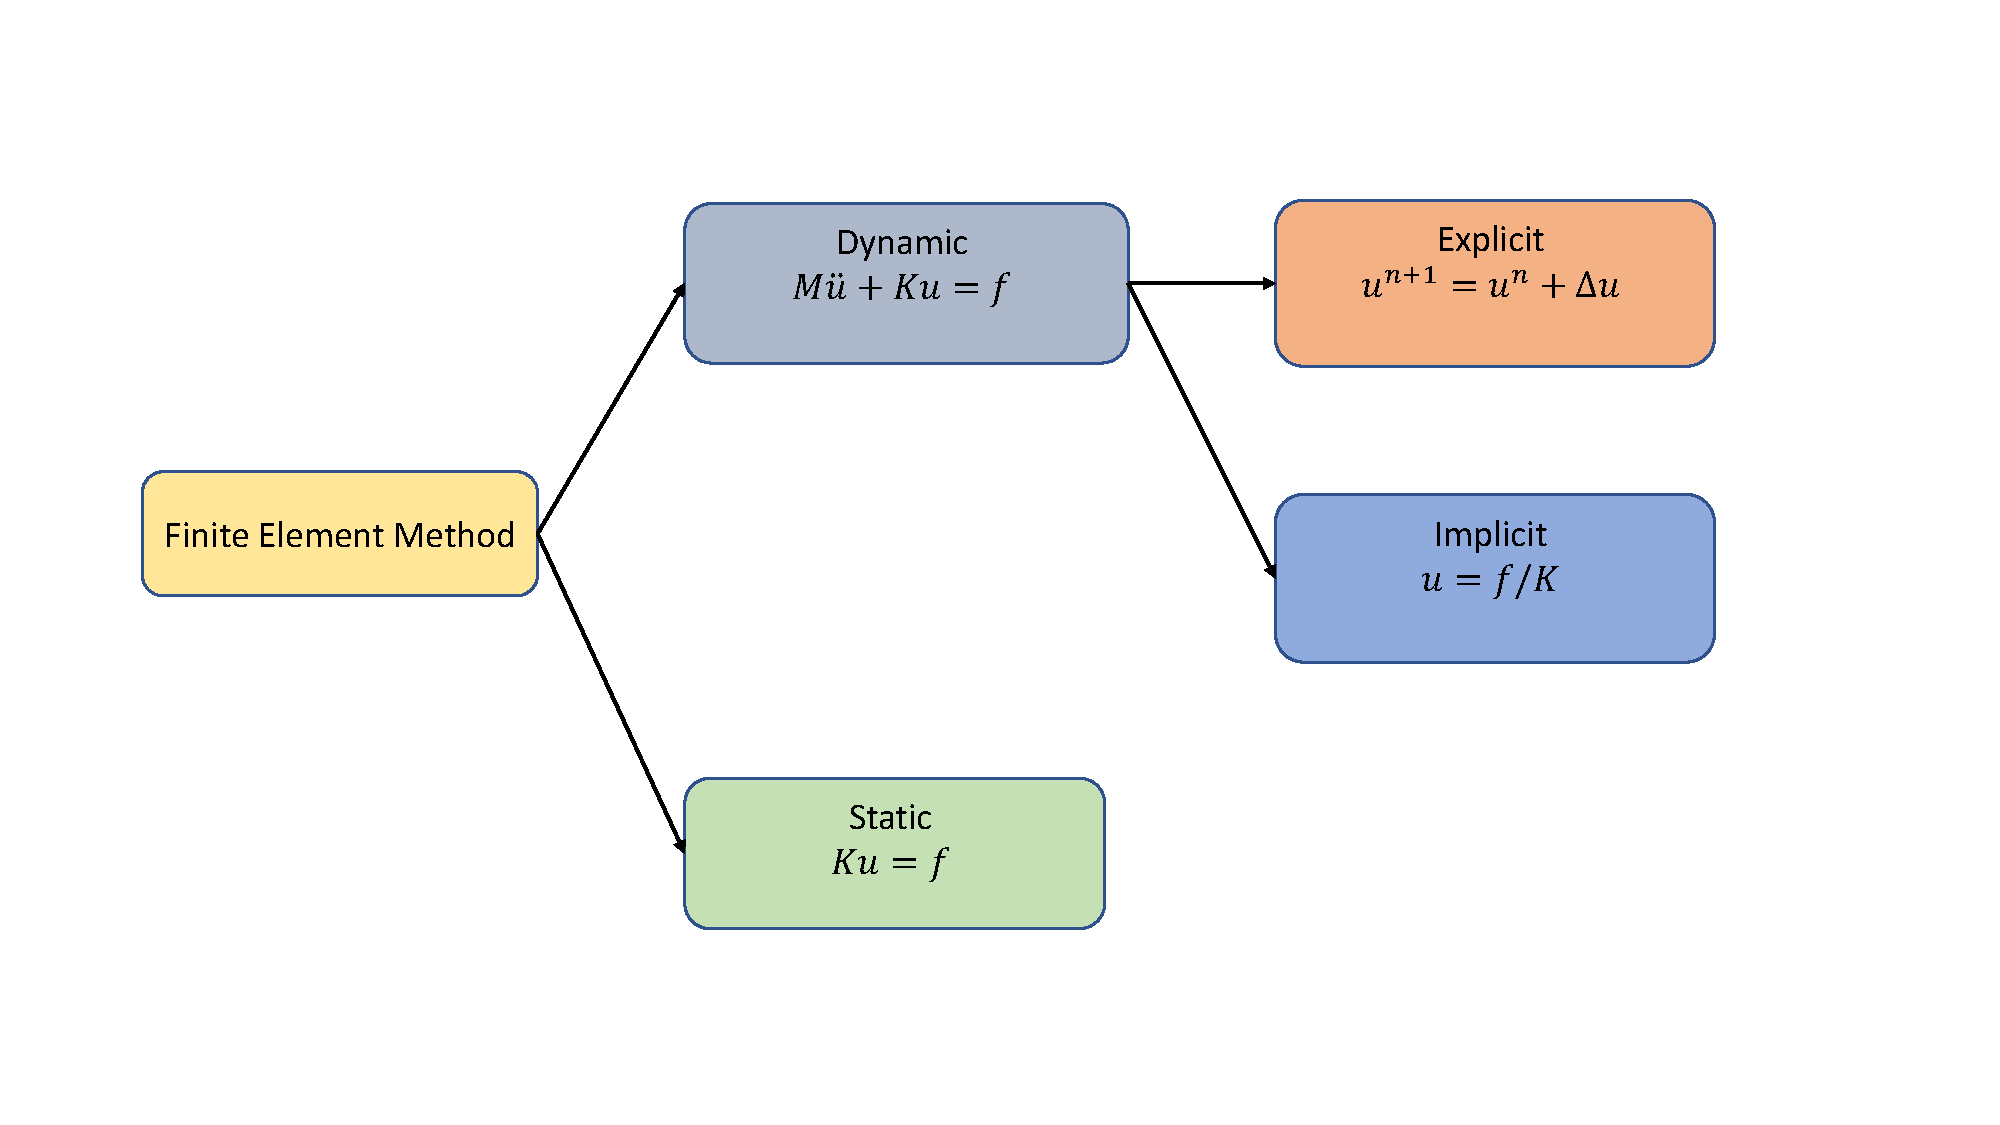
\includegraphics[width=1.0\textwidth]{./pics/fem}
	\end{tabular}
	\caption{\footnotesize Static and dynamic finite element method.} \label{fig: ch1f3}
\end{figure}

The Fig \ref{fig: ch1f3} displays both static analysis and dynamic analysis for a set of linear system of elasticity equations. The steady-state and transient finite element problem are studied with static analysis and dynamic analysis respectively. The latter is time dependent. In dynamic analysis, we shall consider the spatial discretization by using both explicit and implicit time integration schemes\cite{bathe2008finite}. The implicit time marching scheme is computationally costly, since the matrix inversion for large linear system is required every time-step, similar to solving the static problem. The benefit is unconditionally stable for large time step. On the other hand, the explicit time marching scheme requires much lower computational cost as no linear solver is involved for each time-step. However, the size of each time step has to satisfy the numerical stability criteria. 


The linear system of elasticity equations derived from the FEM method is positive definite and too large to be direct inverse. The most time consuming part in the FEM analysis in Fig \ref{fig: ch1f2} is solving the linear system. The complex system can be simplified as a matrix form $ \mathbf{A} \mathbf{x} = \mathbf{b} $. To sovle it, there are two main group of algorithms, directive method and iterative method. Considering the better performance on memory usage and computing time, the iterative method gains more affirmatives\cite{brussino1989comparison} for large scale problems. Preconditioned Conjugate Gradient (PCG) is the one of the most popular method because of its robustness and fast speed. However, Due to the PCG requires positive definite matrix. It is still very challenging to implement finite element analysis using implicit scheme to study the material real-time response behavior. Therefore, the domain decomposition method combined with parallel computing scheme is one emerging choice to tackle that problem.

Parallel computing requires extra effort to tailor the algorithm to achieve concurrent execution. The challenges to reach that purpose include learning and understanding programming paradigms, design the balance load to maximize the usage of bandwidth, minimize the overhead on data communication and synchronization to avoid potential data race problems. In a short conclusion, the high performance computation based on CPU clusters is very challenging dealing with the complex hardware architecture and associated distributed memory. n that case, some modern techniques such as MPI, Intel Math-Kernel library and LAPACK-BLAS can assist us to achieve optimal scalability. The key point for accomplish promising performance is to reduce the overhead latency by employing large number of active processors and ensure the balance of loads on each processor.

\subsection{Numerical Method Review}

The Weak Galerkin Finite Element Method (WG-FEM)is a novel developed, effective numerical method for solving partial differential equations. The WG method is first developed by Dr. Junping Wang and Xiu Ye in 2011, and applied on solving second order elliptic equation\cite{wang2014weak}. The main theory of WG method is to introduce a series of weak operators such as weak gradient, weak divergence and weak curl on the computation of corresponding forms of differential equations. The WG finite element method provides a  brand new perspective to solve numerical problems. It builds up the classic Continuous Galerkin(CG) method to an advanced stage. The WG method can be applied on variety of partial differential equations include second order elliptical equation, elasticity equation\cite{wang2016locking}, Stokes equations \cite{wang2016weak} and Maxwell's equations \cite{mu2013weak}, etc. The WG method inherits the discontinuity from the discontinuous basis functions. The construction of discrete matrix is independent with any external coefficients. The interior unknown variables can be eliminated to the boundary unknown variables to construct a linear system which only consists by degree of freedom(DOFs) along the element boundary. In short, even though the total DOFs of WG method is larger than Discontinuous Galerkin method (DG), the interior unknown variables can eliminated through Schur complement method. The only left DOFs are along the element boundary which are far less than DOFs in DG finite element method. The elemental stiffness matrix of WG method can be constructed upon each element, which is consistent with CG FEM method. 

%-----------------------------------------------------
\section{Objectives of this Work}

The CG FEM analysis of continuum mechanics is widely used to study and predict the material deformation. The results are generally accurate and reliable for analyzing the relationship between load and deformation. However, the computational complexity and cost inhibits the application on conquering the real-time FSI problems. Massive parallel computing is required for obtaining large linear system. In this work, we investigate methods for efficient parallel scheme which enables high-order novel finite element method in solving elasticity equation.

We employ the WG-FEM to convert the bilinear form equations into a positive definite linear system. The WG method has the capacity on varying high-order elements. The selection of polynomials on interior or boundary region is flexible which enhance the freedom on computational simulation. Moreover, the discontinuity features in the WG method which empowers the parallel computation capability.

The Balancing Domain Decomposition by Constraints (BDDC) method is an ideal candidate for entitling the massive parallel capacity to WG-FEM. BDDC identifies the two spaces (primal and dual) to divide and conquer the original computational domain. By minimizing the global communication and synchronization overhead,  WG-BDDC enriches the scalability of elasticity equations as a superlinear speedup curve.

The main objective of this dissertation is to deliver high speed, accuracy and scalability in WG-BDDC based analysis. Fig \ref{fig: ch1p4} shows the paths to accomplish the objectives in this work. The results of the research significantly improves the computation of the elastic material response, including in clinic judgment and other medical applications.

\begin{figure}[H]
	\centering
	\begin{tabular}{c}
		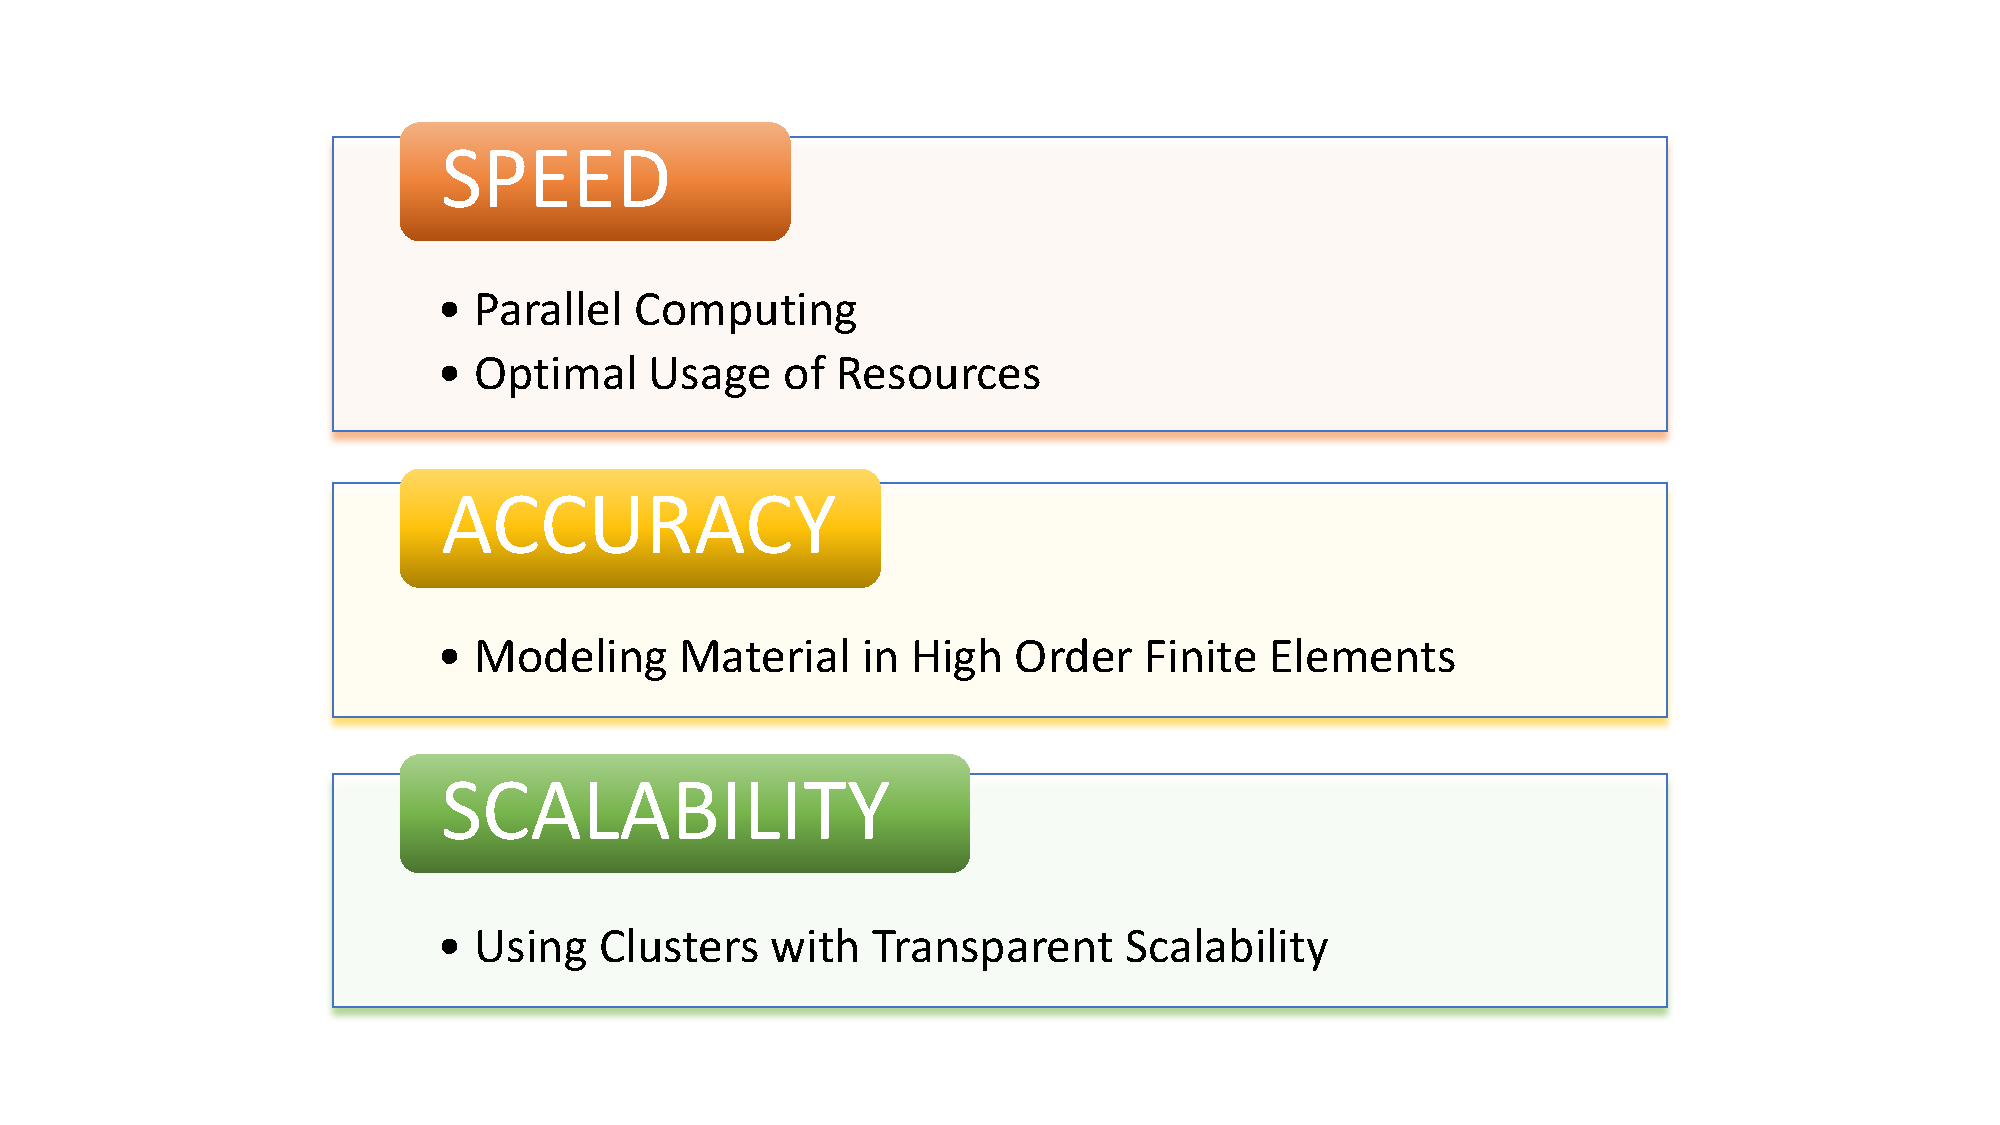
\includegraphics[width=1.0\textwidth]{./pics/ch1p4}
	\end{tabular}
	\caption{\footnotesize Objectives and methodology.} \label{fig: ch1p4}
\end{figure}

To validate the WG-BDDC scheme and develop the software, we first design the hybrid WG-CG element. The results are consistent with the benchmark of CG only element so the fidelity is proved. Then we extend the WG element to BDDC method and verify the properties of convergence and the order of accuracy with parallel fashion. Finally, the scalability is discussed under the parallel computing framework.

The rest of this dissertation is organized as :

\begin{itemize}
	\item Chapter 2 presents the background and basics of WG method.
	\item Chapter 3 discusses the hybrid WG-CG element the performance on nonlinear elasticity equation.
	\item Chapter 4 introduces the WG-BDDC method for second order elliptic and elasticity equation.
	\item Chapter 5 shows the study of effect multiple stenoses on the peripheral artery diseases.
	\item Chapter 6 concludes this work and outlook the future work.
\end{itemize}



\bibliographystyle{elsarticle}
\bibliography{references}

\end{document}
